% Set our document class to Beamer
% \documentclass[aspectratio=169]{beamer}
\documentclass[aspectratio=169, handout]{beamer}
% Add handout option to ignore pauses

% From Jeff E
\usepackage{algo}
% Some more macros
\usepackage{sigmastyle}

% Set a title
\title{Straightening Laws in Algebraic Complexity}

% Set a subtitle if you desire
% \subtitle{Purdue Theory CS/Math Seminar}

% Whoever worked on the presentation:
\author{Anakin Dey}

% Date looks ugly, so leave blank
\date{}

% An institute name, if you're so inclined
% \institute{The Ohio State University}

% Use the SIGma theme for this Beamer presentation
\usetheme{sigma}
% --------------------------------------------------------------------

% one-offs
\newcommand{\svdots}{\raisebox{-0.12\height}[0pt][0pt]{$\vdots$}}
\newcommand{\ra}{r_1}
\newcommand{\rb}{r_2}
\newcommand{\rd}{r_d}
\newcommand{\ca}{c_1}
\newcommand{\cb}{c_2}
\newcommand{\cd}{c_d}

\DeclareMathOperator{\pfaff}{pfaff}
\DeclareMathOperator{\sym}{sym}

\makeatletter
\DeclareRobustCommand\bigop[1]{%
  \mathop{\vphantom{\cdot}\mathpalette\bigop@{#1}}\slimits@
}
\newcommand{\bigop@}[2]{%
  \vcenter{%
    \sbox\z@{$#1\sum$}%
    \hbox{\resizebox{\ifx#1\displaystyle.9\fi\dimexpr\ht\z@+\dp\z@}{!}{$\m@th#2$}}%
  }%
}
\makeatother

\newcommand{\Sub}{\DOTSB\bigop{\mathrm{Sub}}}

% Begin document
\begin{document}

\begin{frame}
\titlepage
\end{frame}

% Will determine later if I want TOC or even section frames
% \begin{frame}{Outline}
%   \tableofcontents
% \end{frame}

\section{Background}
\frame{\sectionpage}

\begin{frame}{What is Algebraic Complexity?}
    \only<1>{
    \vspace{25pt}
    \begin{question}
        How hard is it to compute polynomials?
    \end{question}
    }
    \onslide<2->{
    \begin{question}
        How hard is it to compute polynomials in restricted models?
    \end{question}
    }
    
    \onslide<3>{
    \begin{question}
        Can we find \emph{explicit} polynomials which are hard to compute?
    \end{question}
    }
\end{frame}

\begin{frame}{Algebraic Circuits}
    \begin{minipage}[c]{0.5\textwidth}
        \begin{figure}
            \centering
            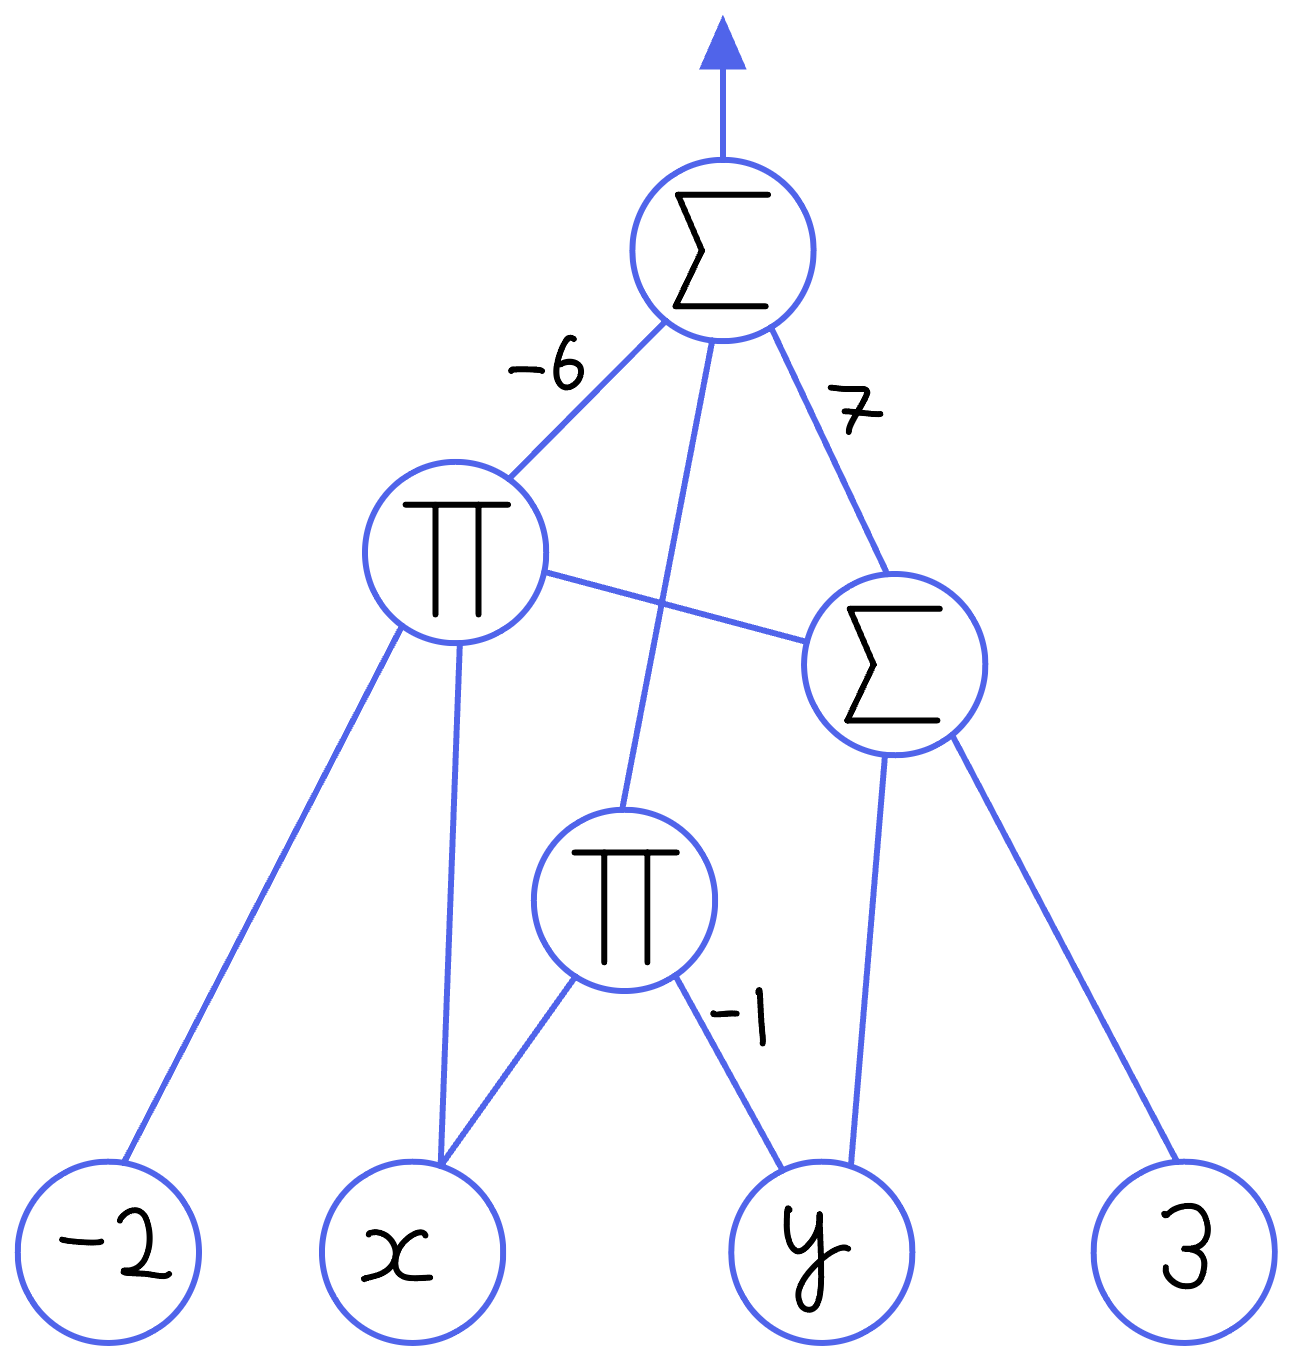
\includegraphics[width=\textwidth]{images/ckt.png}
            \caption{$-6(-2x \cdot (y + 3)) -xy + 7(y + 3)$}
        \end{figure}
    \end{minipage}% 
    \begin{minipage}[c]{0.5\textwidth}
        \pause

        We have two measures of complexity: \pause
        \begin{itemize}
            \item \emph{Size:} The number of edges \pause
            \item \emph{Depth:} The length of the longest input-output path
        \end{itemize}
    \end{minipage}
\end{frame}

\begin{frame}{Horner's Rule}

\end{frame}

\begin{frame}{Hard Polynomials Exist}

\end{frame}

\begin{frame}{Border Complexity}
    One relaxation in algebraic complexity is to \emph{approximate} a polynomial.

    \pause
    \vspace{10pt}

    Instead of working over a field $\F$\pause, we take a parameter $\e$, allow our coefficients to be rational functions in $\e$, and let $\e$ tend to $0$.

    \pause
    \vspace{10pt}
    
    \begin{defn}
    We say a circuit \emph{border computes} $g(\overline{x})$ over $\F$ if it computes
    \[
        g(\overline{x}) + \varepsilon^q \tilde{g}(\overline{x}, \varepsilon) \in \mathbb{F}(\varepsilon)[\overline{x}], \qquad q \geq 1.
    \]
    \end{defn}

    \pause

    We \textcolor{sigma@alertred}{cannot} set $\e = 0$ since we may divide by $\e$.
\end{frame}

\begin{frame}{What does Border Computation Get Us?}
    \begin{question}
        What is the power of border computation?

        \pause
        \vspace{20pt}

        Is it strictly necessary? \pause
        Can we prove something in the border setting and \emph{deborder} the result to get an exact computation?
    \end{question}    
\end{frame}

\begin{frame}{Circuit Complexity for Ideals}
    \pause
  
    In algebraic complexity, we are interested in characterizing the \emph{circuit complexity} of some family of polynomials.

    \pause

    \begin{defn}
        Fix some polynomials $g_1(\overline{x}), \ldots, g_k(\overline{x}) \in \mathbb{F}[\overline{x}]$.

        \pause
        
        The \emph{ideal} generated by $g_1(\overline{x}), \ldots, g_k(\overline{x})$ is the set of combinations
        \[
            \gen{g_1, \ldots, g_k} = \Set{\sum_{i = 1}^k h_i(\overline{x}) \cdot g_i(\overline{x}) \quad \Bigg| \quad h_i(\overline{x}) \in \F[\overline{x}]}.
        \]
    \end{defn}

    \pause
    
    \begin{question}
        Suppose $f \in \gen{g_1, \ldots, g_k}$.\ \pause
        How does the complexity of $f$ compare to the complexity of the generators $g_1, \ldots, g_k$?
    \end{question}
\end{frame}

\begin{frame}{Algebraic Circuits with Oracles}
    \onslide<3>{
    \begin{minipage}[c]{0.5\textwidth}
        \begin{figure}
            \centering
            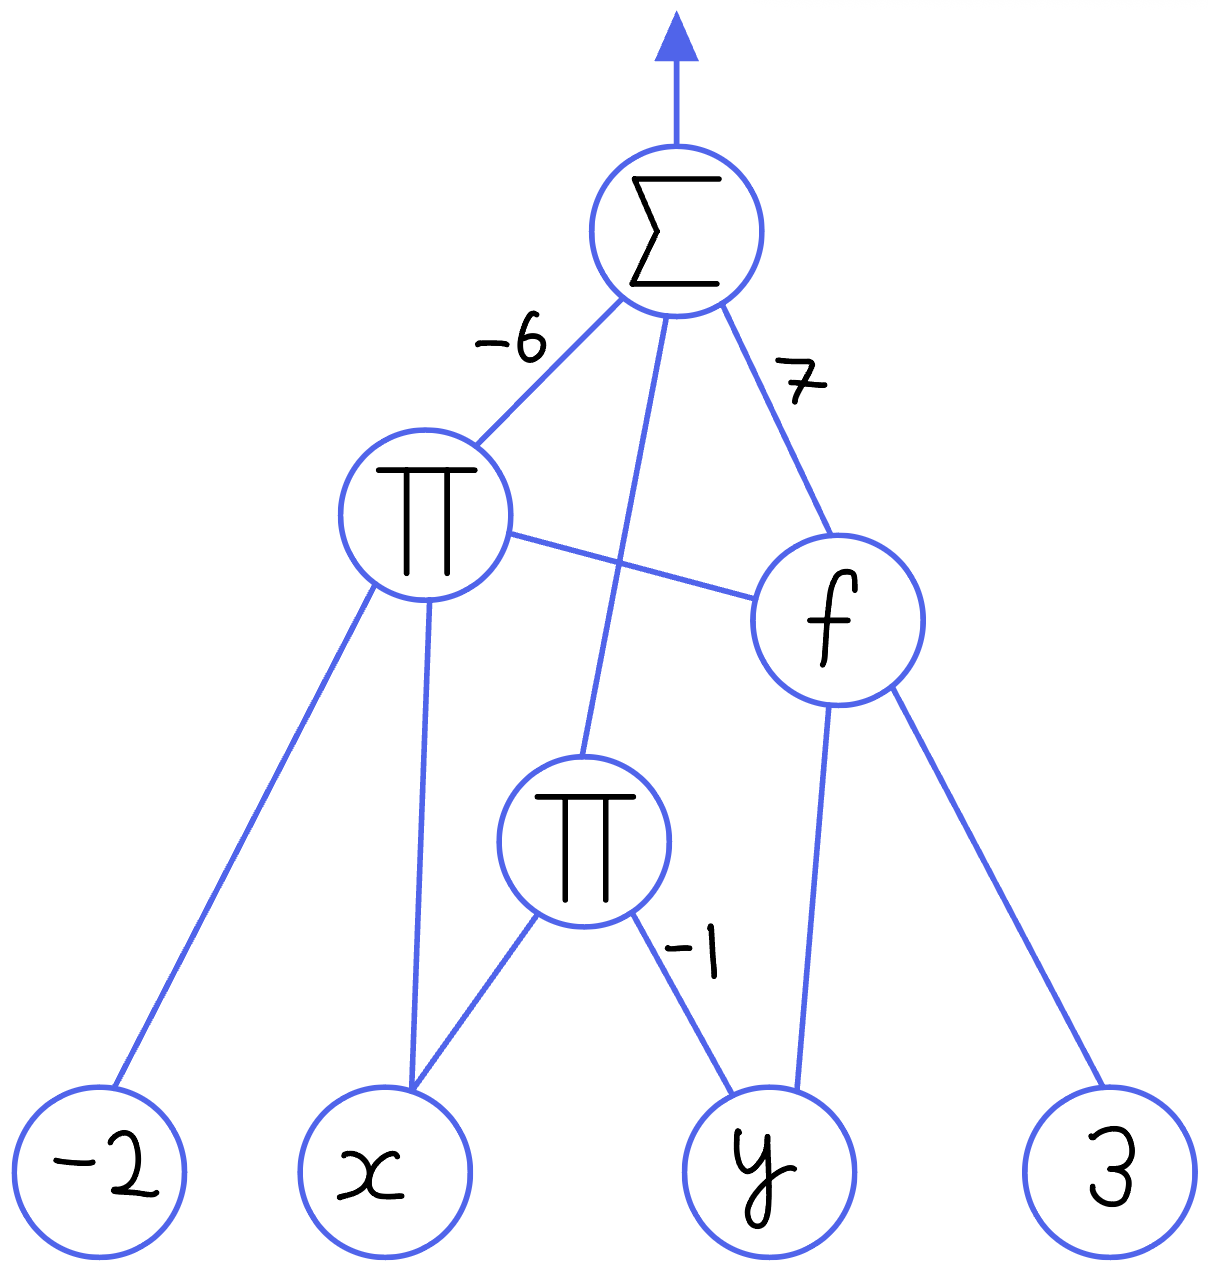
\includegraphics[width=0.99375\textwidth]{images/oracle-ckt.png}
            \caption{$-6(-2x \cdot f(y, 3)) -xy + 7f(y, 3)$}
        \end{figure}
    \end{minipage}}%
    \begin{minipage}[c]{0.5\textwidth}
        \pause

        \begin{question}
            How can we compare the \emph{relative} \linebreak complexity of two polynomials?
        \end{question}

        \pause
        \vspace{30pt}

        We can allow a fixed polynomial $f(\overline{x})$ to be computed with unit cost by allowing it to function as its own gate.
    \end{minipage}
\end{frame}

\begin{frame}{Principal Ideals}
    \begin{ex}
        The \emph{principal ideals} are generated by a single polynomial $g$.

        \pause
        \vspace{10pt}
        
        If $f \in \gen{g}$,\ \pause then $g$ is a \emph{factor} of $f$.
    \end{ex}

    \pause
    \vspace{20pt}
    
    \begin{question}
        Suppose $f \in \gen{g}$.
        Does $g$ have a small $f$-oracle circuit?
    \end{question}
\end{frame}

\begin{frame}{Principal Ideals}
    \begin{conj}[{\cite[Conjecture 8.3]{Burgisser2000}}]
        If $g$ is a factor of $f$, $\size(g) \leq \poly(\size(f), \deg(f))$.
    \end{conj}

    \pause

    \begin{thrm}[{\cite[Theorem 1.3]{Burgisser2004}}]
        Over fields of characteristic $0$, $g$ can be \emph{border computed} by a circuit of size $\poly(\size(f), \deg(f))$.
    \end{thrm}

    \pause
    \vspace{10pt}

    \begin{question}
    Can we \emph{deborder} this result, that is can we remove this $\e$ approximation?
    \end{question}
\end{frame}

\begin{frame}{What about Two Generators?}
    Consider an ideal with two generators $\ideal{g_1(\overline{x}), g_2(\overline{x})}$.

    \pause

    Say $0 \neq f(\overline{x}) \in \ideal{g_1(\overline{x}), g_2(\overline{x})}$: \pause
    \[
      f(\overline{x}) = h_1(\overline{x}) g_1(\overline{x}) + h_2(\overline{x}) g_2(\overline{x}). \pause
    \]
    \begin{question}
      If $f(\overline{x})$ has a small circuit, do $g_1(\overline{x})$ or $g_2(\overline{x})$ have a small $f$-oracle circuit? 
    \end{question}

    \pause

    This is open for \emph{general} polynomials $g_1(\overline{x}), g_2(\overline{x})$~\cite{Gro20}.
\end{frame}

\begin{frame}{Determinantal Ideals}
    Questions about oracle circuit complexity are open for general ideals with more than one generator.\ \pause
    We can instead ask about ideals whose generators have \emph{additional structure}.

    \pause
    \vspace{10pt}
    
    \begin{ex}
        Consider an $n \times m$ matrix $X = (x_{i, j})$ of variables.\ \pause
        Let $I_{n, m, r}^{\det}$ be the \emph{determinantal ideal} generated by the $r \times r$ minors of $X$.
    \end{ex}
\end{frame}

\begin{frame}{Prior Closure Results in Determinantal Ideals}
    \begin{ex}
        Consider an $n \times m$ matrix $X = (x_{i, j})$ of variables.
        Let $I_{n, m, r}^{\det}$ be the \emph{determinantal ideal} generated by the $r \times r$ minors of $X$.
    \end{ex}

    \pause
    
    \begin{conj}[{\cite[Conjecture 6.3]{Gro20}}]
        Let $f \in I^{\det}_{n, n, n / 2}$ be a nonzero polynomial.\ \pause
        There is a constant depth $f$-oracle circuit of size $\poly(n)$ that computes the $t \times t$ determinant, $t = n^{\bigTheta{1}}$.
    \end{conj}
\end{frame}

\begin{frame}{What does the Oracle Give Us?}
    \begin{conj}[{\cite[Conjecture 6.3]{Gro20}}]
        Let $f \in I^{\det}_{n, n, n / 2}$ be a nonzero polynomial.
        There is a constant depth $f$-oracle circuit of size $\poly(n)$ that computes the $t \times t$ determinant, $t = n^{\bigTheta{1}}$.
    \end{conj}

    \pause
    \vspace{10pt}

    \begin{itemize}
        \item There exist polynomial size circuits for computing $\det(X)$.\pause
        \item However, these circuits are \emph{not} constant-depth.\pause
        \item The oracle allows \emph{constant depth} computation of the determinant.
    \end{itemize}
\end{frame}

\begin{frame}{Closure Results in Determinantal Ideals}    
    \begin{thrm}[{\cite[Theorem 1.1]{AF22}}]
        Let $f \in I^{\det}_{n, m, r}$ be a nonzero polynomial.
        Then there is a depth-three $f$-oracle circuit of size $\bigO{n^2 m^2}$ that \emph{border computes} the $t \times t$ determinant for some $t = \bigTheta{r^{1 / 3}}$.
    \end{thrm}

    \pause

    \begin{question}
        Can we \emph{deborder} this result, that is can we remove this $\e$ approximation?
    \end{question}
\end{frame}

\begin{frame}{Closure Results in Determinantal Ideals}
    \begin{thrm}[{\cite[Theorem 1.5]{DG25}}]
        Let $f \in I^{\det}_{n, m, r}$ be a nonzero polynomial.
        Then there is a depth-three $f$-oracle circuit of size $\poly(n, m, \deg(f))$ that \emph{exactly computes} the $t \times t$ determinant for some $t = \bigTheta{r^{1 / 3}}$.
    \end{thrm}

    \pause

    Main Tools:
    \begin{itemize}
        \item We use \emph{Straightening Laws} from Invariant Theory to express $f(X)$ in a standard basis indexed by Young tableau, \pause and leverage the combinatorics to talk about specific terms.\pause
        \item To get a circuit for a specific basis term, we use \emph{Homogenization} as well as a new application of the \emph{Isolation Lemma}.
    \end{itemize}
\end{frame}

\section{Preliminaries}
\frame{\sectionpage}

\begin{frame}{Bideterminants}
    \begin{defn}[Bideterminants]
        Let $\sigma = (4, 2, 1)$.\ \pause
        Consider the \emph{bitableau} $(S \mid T)$ of shape $\sigma$
        \[
            (S \mid T) = \left(\ \Yvcentermath1 \left. \young(1245,36,4)\ \right\vert\ \young(1356,27,3) \ \right).
        \]

        \pause
        
        Then the \emph{bideterminant} $(S \mid T)(X)$ is given by
        \[
            (S \mid T)(X) = 
            \begin{pmatrix}
                x_{1, 1} & x_{1, 3} & x_{1, 5} & x_{1, 6} \\
                x_{2, 1} & x_{2, 3} & x_{2, 5} & x_{2, 6} \\
                x_{4, 1} & x_{4, 3} & x_{4, 5} & x_{4, 6} \\
                x_{5, 1} & x_{5, 3} & x_{5, 5} & x_{5, 6} 
            \end{pmatrix}
            \begin{pmatrix}
                x_{3, 2} & x_{3, 7} \\
                x_{6, 2} & x_{6, 7}
            \end{pmatrix}
            \begin{pmatrix}
                x_{4, 3}
            \end{pmatrix}.
        \]
    \end{defn}
\end{frame}

\begin{frame}{A Natural Generating Set for Determinantal Ideals}
    \begin{lem}
        A degree $d$ monomial $\prod_{i = 1}^d x_{r_i, c_i}$ is given by a bideterminant: \pause
        \[
    	      \prod_{i = 1}^d x_{r_i, c_i} = \left(\ \Yvcentermath1 \left.\young(\ra,\rb,\svdots,\rd) \ \right\vert\ \young(\ca,\cb,\svdots,\cd) \ \right)(X).
        \]
    \end{lem}
    \pause
    Thus, the bideterminants span $\F[X]$.
\end{frame}

\begin{frame}{A Natural Generating Set for Determinantal Ideals}
  \begin{thrm}[{\cite[\S 8, Theorem 3]{DRS74},~\cite[Corollary 2.3]{dCEP80}}]
    Let $(S \mid T)(X)$ be a bideterminant of shape $\sigma$.
    \pause
    Then $(S \mid T)(X)$ can be uniquely expressed as a linear combination
    \[
        (S \mid T)(X) = \sum_{(A \mid B)} c_{A, B} (A \mid B)(X),
    \]
    where $A$ and $B$ are \emph{conjugate semistandard}.
  \end{thrm}

  \pause

  Since $I^{\det}_{n, m, r}$ is generated by the $r \times r$ minors, the bideterminants in our basis should have at least one determinant of length at least $r$.

  \pause
  
  \begin{prop}[{\cite[Corollary 1.7]{BC03}}]
    The ideal $I^{\det}_{n, m, r}$ has as basis the conjugate semistandard bideterminants of shape $\sigma$ whose first row has length at least $r$.
  \end{prop}
    
\end{frame}

\begin{frame}{Shuffle Products}

\end{frame}

\begin{frame}{Laplace Expansion}

\end{frame}

\begin{frame}{Example Straightening}

\end{frame}

\begin{frame}{Proof of Grochow's Conjecture Given Theorem}
    \begin{conj}[{\cite[Conjecture 6.3]{Gro20}}]
        Let $f \in I^{\det}_{n, n, n / 2}$ be a nonzero polynomial.
        Then there is a constant depth $f$-oracle circuit of size $\poly(n)$ that computes the $t \times t$ determinant for some $t = n^{\bigTheta{1}}$.
    \end{conj}

    \pause
    
    \begin{thrm}[{\cite[Theorem 1.5]{DG25}}]
        Let $f \in I^{\det}_{n, m, r}$ be a nonzero polynomial.
        Then there is a depth-three $f$-oracle circuit of size $\poly(n, m, \deg(f))$ that \emph{exactly computes} the $t \times t$ determinant for some $t = \bigTheta{r^{1 / 3}}$.
    \end{thrm}
\end{frame}

% Formal ABP Definition
% \begin{frame}{Algebraic Branching Programs}
%     \begin{defn}
%         An \emph{algebraic branching program} (\emph{ABP}) over $\F$ is a directed acyclic graph $A$ such that:
%         \begin{itemize}
%             \item The nodes $V$ of $A$ are partitioned into non-empty subsets $V = V_0 \sqcup \cdots \sqcup V_d$ for some integer $d\geq 0$ and we call $V_i$ the \emph{$i$-th layer}.
%                   Layer $V_0$ has exactly one node called the \emph{source $s$} and layer $V_d$ has exactly on node called the \emph{sink $t$}.
%             \item Each edge in $A$ goes from layer $V_{i-1}$ to $V_i$ for some $i\in [d]$.
%             \item Each edge $e$ in $A$ is labeled with a polynomial $\gamma_e \in \F[\overline{x}]$ of degree at most one.
%         \end{itemize}
%         For a path $\overline{e} = (e_1, \ldots, e_d)$ from $s$ to $t$, where each edge $e_i$ goes from layer $i - 1$ to layer $i$, define the polynomial $\gamma_{\overline{e}} \defeq \prod_{i = 1}^d \gamma_{e_i}$.
%         Then $A$ computes the polynomial $\sum_{\text{path } \overline{e} \text{ from } s \text{ to } t} \gamma_{\overline{e}}$.
%     \end{defn}   
% \end{frame}

\begin{frame}{Main Theorem}
    \begin{thrm}
        Let $f(X) \in I^{\det}_{n, m, r}$ be a nonzero polynomial of degree $d$.
        Then, there exists a depth-three $f$-oracle circuit of size $\bigO{n^2m^2d^3(n^3+m^3)}$ computing $(K_\sigma \mid K_\sigma)(X)$, where $\sigma_1 \geq r$ and $\abs{\sigma} \leq d$.
    \end{thrm}

    \pause
    
    Let $\sigma = (4, 2, 1)$:
    \begin{align*}
      (K_\sigma \mid K_\sigma)(X) &= \left(\ \Yvcentermath1 \left. \young(1234,12,1)\ \right\vert\ \young(1234,12,1) \ \right)(X) \\
                                  &= \text{product of upper-left minors}.
    \end{align*}
\end{frame}

\section{Proof Techniques}
\frame{\sectionpage}

\begin{frame}{Proof Outline}
    Since we are starting with $f(X) \in I^{\det}_{n, m, r} \subseteq \F[X]$,\ \pause we can express in terms of our standard basis:
    \[
        f(X) = \sum_{k \in I} c_k (S_k \mid T_k)(X).
    \]

    \pause
    
    Our goal will be to use $f(X)$ as an oracle to compute a canonical bideterminant.

    \pause
    
    To do this, we will isolate one of the terms $(S_k \mid T_k)(X)$.
  \end{frame}
  
\begin{frame}{Linear Operators}
    \begin{defn}[Substitution operator]
        For $i < j$, the operator $\mathrm{Sub}_{i \to j}$ takes a tableau $S$ and returns the tableau $S'$ formed by taking each row of $S$ which has an $i$ but not a $j$, replacing that $i$ with $j$, and sorting the row in increasing order.

        \pause
        
        \[
            \Yvcentermath1 \Sub_{2 \to 4} \young(1234,12,1)\ =\ \young(1234,14,1)
        \]

        \pause
        
        Let $h_{i}^{j}(S)$ be the number of times $i$ is replaced by $j$ in $S$.
    \end{defn}
\end{frame}

\begin{frame}{Linear Operators}
    These operators send conjugate semistandard tableau to conjugate semistandard tableau.

    \pause
    
    In fact, after enough applications we arrive at \emph{anticanonical} tableau: \pause
    \begin{lem}[{\cite[stated before Corollary 1.7]{dCEP80}}]
        Let $S$ be a conjugate semistandard tableau of shape $\sigma$ such that $S$ has entries of value at most $n$.
        \pause
        Then
        \begin{align*}
          (\Sub_{n - 1 \to n} &\circ \Sub_{n - 2 \to n} \circ \Sub_{n - 2 \to n-1} \circ \cdots \\
          &\circ \Sub_{2 \to n}\circ\cdots\circ\Sub_{2 \to 3} \circ \Sub_{1 \to n} \circ \cdots \circ \Sub_{1 \to 2})(S) = \overline{K}_\sigma.
        \end{align*}
    \end{lem} 
\end{frame}

\begin{frame}{Linear Operators}
    \begin{lem}[{\cite[stated before Corollary 1.7]{dCEP80}}]
        Let $S$ be a conjugate semistandard tableau of shape $\sigma$ such that $S$ has entries of value at most $n$.
        Then
        \begin{align*}
          (\Sub_{n - 1 \to n} &\circ \Sub_{n - 2 \to n} \circ \Sub_{n - 2 \to n-1} \circ \cdots \\
          &\circ \Sub_{2 \to n}\circ\cdots\circ\Sub_{2 \to 3} \circ \Sub_{1 \to n} \circ \cdots \circ \Sub_{1 \to 2})(S) = \overline{K}_\sigma.
        \end{align*}
    \end{lem} 

    \pause

    \begin{ex}
        Say $n = 5$
        \begin{align*}
            \Yvcentermath1 \young(1234,12,1)\qquad \onslide<3>{\rightsquigarrow \qquad \young(2345,45,5)}
        \end{align*}
    \end{ex}
\end{frame}

\begin{frame}{Applying the Linear Operators}
    Substituting $i$ for $j$ corresponds to multiplication of $X$ by an \emph{elementary matrix} $E_{i, j}$, adding a multiple of row $j$ to row $i$.
    
    \pause
  
    \begin{lem}
        Let $\lambda$ be a new indeterminate and let $(S \mid T)$ be a bitableau.\ \pause
        Then we have that
        \[
            (S \mid T)(E_{i, j}(\lambda)X) \pause = \pm \lambda^{h_{i}^{j}(S)} (\Sub_{i \to j}(S) \mid T)(X) \pause + \sum_{h = 0}^{h_{i}^{j}(S) - 1} \lambda^h \sum_{S' \in \mathcal{C}^{h}_{i \to j}(S)} \pm  (S' \mid T)(X).
        \]
        For $0 \leq h \leq h_{i}^{j}(S) - 1$, let $\mathcal{C}^{h}_{i \to j}(S)$ be the set of tableaux of shape $\sigma$ obtained by changing $i$ to $j$ at exactly $h$ rows of $S$ which contain $i$ but not $j$ and reordering those rows to be increasing.
    \end{lem}
\end{frame}

\begin{frame}{Applying the Linear Operators}
    We have seen now that after applying a sequence of linear transformations $E_{i, j}$ to our matrix of variables $X$, we can send a bitableau $(S \mid T)$ of shape $\sigma$ to $(\overline{K}_\sigma \mid \overline{K}_\sigma)$.

    \pause
    \vspace{20pt}

    Let $J_n$ be the $n \times n$ matrix with $1$'s along the anti-diagonal.\ \pause
    \begin{lem}
        \[
            (\overline{K}_\sigma \mid \overline{K}_\sigma)(J_n X J_m) = \pm (K_\sigma \mid K_\sigma)(X).
        \]
    \end{lem}

    \pause
    \vspace{20pt}

    We now have linear transformations sending bitableau to canonical semistandard Young tableau.
\end{frame}

\begin{frame}{Where Does Isolation Arise?}
  \[
    f(X) = \sum_{k \in I} c_k (S_k \mid T_k)(X) \in I^{\det}_{n, m, r}.
  \]

  \pause
  \vspace{20pt}

  \begin{cor}
      We have matrices $M, N$ such that
      \begin{equation*}
              f(M X N) = \sum_{k \in A} \widehat{c}_{k} \Lambda^{\overline{e}_k}\Xi^{\overline{f}_k}\cdot (K_{\sigma_k}\mid K_{\sigma_k})(X) + \sum_{\ell \in B} \widehat{c}_{\ell} \Lambda^{\overline{e}_\ell}\Xi^{\overline{f}_\ell}\cdot (S_\ell\mid T_\ell)(X),
      \end{equation*}
  \end{cor}

  \pause
  Upshot: linear transformations correspond to plugging in linear equations into the input for $f(X)$, \pause so this is the start of our $f$-oracle circuit.
\end{frame}

\begin{frame}{Where Does Isolation Arise?}
  \[
    f(X) = \sum_{k \in I} c_k (S_k \mid T_k)(X) \in I^{\det}_{n, m, r}, \qquad \deg(f) = d.
  \]

  \vspace{20pt}

  \begin{cor}
      We have matrices $M, N$ such that
      \begin{equation*}
              f(M X N) = \sum_{k \in A} \widehat{c}_{k} \Lambda^{\overline{e}_k}\Xi^{\overline{f}_k}\cdot {\color{sigma@mainblue}(K_{\sigma_k}\mid K_{\sigma_k})(X)} + \sum_{\ell \in B} \widehat{c}_{\ell} \Lambda^{\overline{e}_\ell}\Xi^{\overline{f}_\ell}\cdot (S_\ell\mid T_\ell)(X),
      \end{equation*}
  \end{cor}
\end{frame}

\begin{frame}{Homogenization}
   \begin{defn}
        Consider a degree $d$ polynomial $g(\overline{x}, t) = \sum_{i = 0}^d \coeff_{t^i}(g) t^i$.
        
        \vspace{-10pt}
    \end{defn} 

    \pause

    \begin{lem}[Folklore]
        Say $g$ is computed by a size $s$, depth $\Delta$ $f$-oracle circuit with top $\Sigma$-gate.

        \pause
        
        \begin{minipage}[c]{0.45\textwidth}
            \begin{figure}
                \centering
                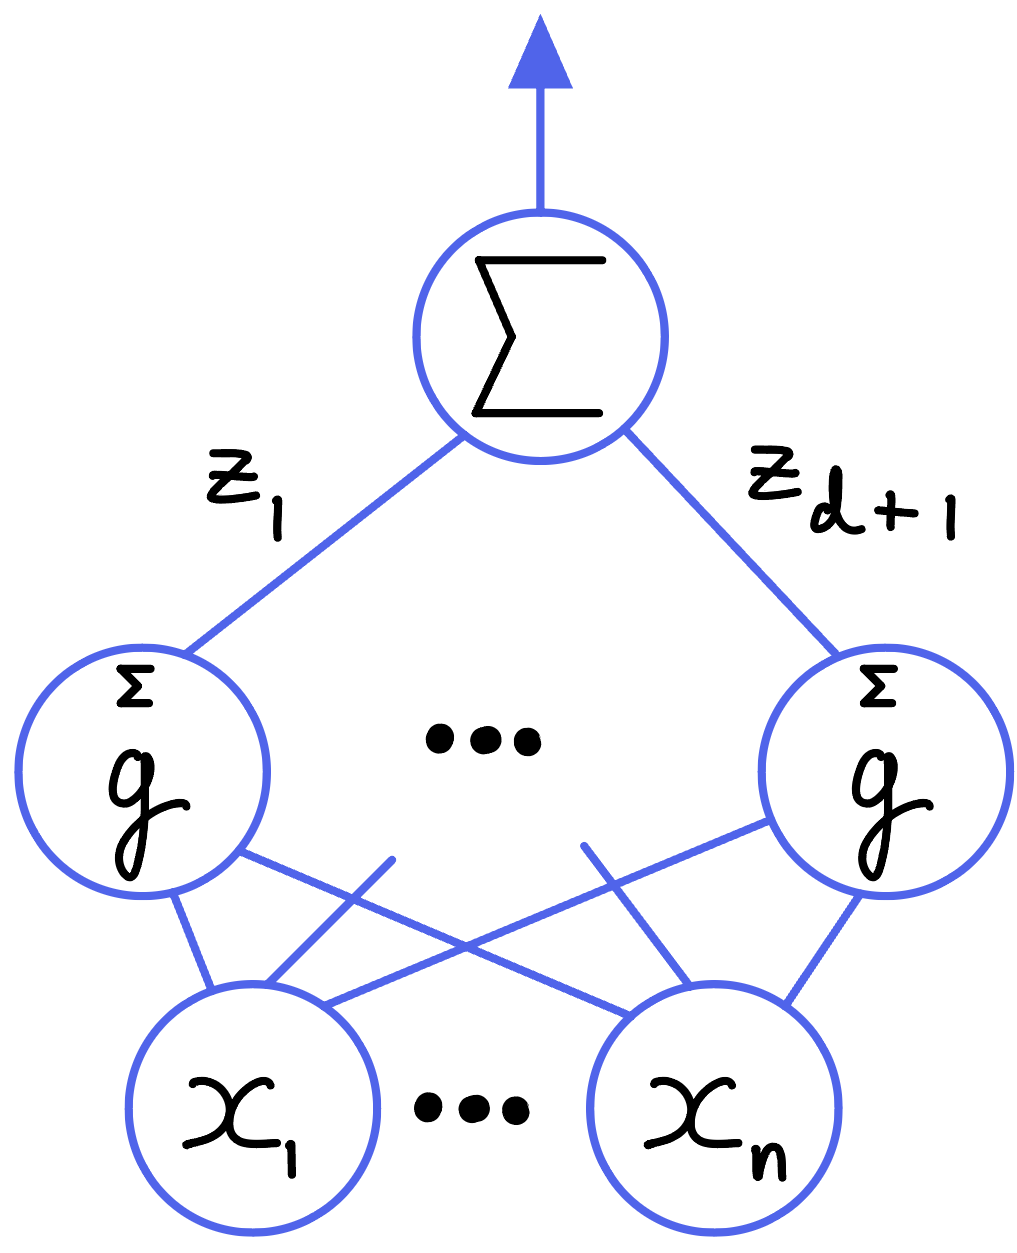
\includegraphics[width=0.625\textwidth]{images/homog.png}
            \end{figure}
        \end{minipage}% 
        \begin{minipage}[c]{0.55\textwidth}
            Then, we can compute $\coeff_{t^i}(g)$ by a size $\bigO{ds}$, depth $\Delta$ $f$-oracle circuit.
        \end{minipage}

    \end{lem}
\end{frame}

\begin{frame}{Proof of Homogenization: Interpolation}
    Let $\alpha_1, \ldots, \alpha_{d + 1}$ be $d + 1$ distinct elements in $\mathbb{F}$.
    \[
        \begin{pmatrix}
            \alpha_1^d & \alpha_1^{d - 1} & \cdots & \alpha_1 & 1 \\ 
            \alpha_2^d & \alpha_2^{d - 1} & \cdots & \alpha_2 & 1 \\ 
            \vdots & \vdots & \ddots & \vdots & \vdots \\
            \alpha_{d}^d & \alpha_{d}^{d - 1} & \cdots & \alpha_{d} & 1 \\ 
            \alpha_{d + 1}^d & \alpha_{d + 1}^{d - 1} & \cdots & \alpha_{d + 1} & 1 
        \end{pmatrix}
        \begin{pmatrix}
            \coeff_{t^d}(f) \\
            \coeff_{t^{d-1}}(f) \\
            \vdots \\
            \coeff_{t}(f) \\
            \coeff_{1}(f)
        \end{pmatrix}
        =
        \begin{pmatrix}
            f(\overline{x},\alpha_1) \\
            f(\overline{x},\alpha_2) \\
            \vdots \\
            f(\overline{x},\alpha_d) \\
            f(\overline{x},\alpha_{d+1})
        \end{pmatrix}        
    \]

    \pause

    This left matrix is a \emph{Vandermonde} matrix and is invertible since the $\alpha_i$ are all distinct.
\end{frame}

\begin{frame}{Proof of Homogenization: Interpolation}
    \[
        \begin{pmatrix}
            \coeff_{t^d}(f) \\
            \coeff_{t^{d-1}}(f) \\
            \vdots \\
            \coeff_{t}(f) \\
            \coeff_{1}(f)
        \end{pmatrix}
        =
        \begin{pmatrix}
            z_{1, 1} & z_{1, 2} & \cdots & z_{1, d} & z_{1, d + 1} \\
            z_{2, 1} & z_{2, 2} & \cdots & z_{2, d} & z_{2, d + 1} \\
            \vdots & \vdots & \ddots & \vdots & \vdots \\
            z_{d, 1} & z_{d, 2} & \cdots & z_{d, d} & z_{d, d + 1} \\
            z_{d + 1, 1} & z_{d + 1, 2} & \cdots & z_{d + 1, d} & z_{d + 1, d + 1} \\
        \end{pmatrix}
        \begin{pmatrix}
            f(\overline{x},\alpha_1) \\
            f(\overline{x},\alpha_2) \\
            \vdots \\
            f(\overline{x},\alpha_d) \\
            f(\overline{x},\alpha_{d+1})
        \end{pmatrix} 
    \]

    \pause

    \begin{equation*}
        \coeff_{t^i}(f) = \sum_{j = 1}^{d + 1} z_{d + 1 - i, j} f(\overline{x},\alpha_j).
    \end{equation*}
\end{frame}

 
% \begin{frame}{Aside: Interpolation in Border Setting}
%     
% \end{frame}

\begin{frame}{Issues with Homogenization}
    If a circuit border computes $g(\overline{x})$, then it computes
    \[
      g(\overline{x}) + \e^q \tilde{g}(\overline{x}, \e), \qquad q \geq 1.
    \]

    \pause
    \vspace{10pt}
    
    \emph{Idea:} Homogenize with respect to $\varepsilon$.
    
    \pause
    \vspace{10pt}
    
    \emph{Problem:} $q$ can be \emph{arbitrarily large} 

    \pause
    
    \qquad $\implies$ Homogenization gives \emph{large circuit}.
\end{frame}

\begin{frame}{Idea: Kronecker Substitution}
    Say there is a specific coefficient $c_{\overline{e}}$ in $g(\overline{x}) = \sum_{\overline{e} \in \mathcal{L}} c_{\overline{e}} {\overline{x}}^{\overline{e}}$ we want to \emph{isolate}.

    \pause
    
    \begin{lem}
        Suppose that $\deg(g) \leq d$, \pause then the \emph{Kronecker substitution}
        \[
            x_i \mapsto w^{d^i}
        \]
        maps distinct monomials to distinct monomials.
    \end{lem}

    \pause

    \emph{Problem:} The resulting polynomial has \emph{large degree}.

    \pause
    
    \qquad $\implies$ Homogenization gives \emph{large circuit}.
\end{frame}

\begin{frame}{Isolation Lemma}
    Say there is a specific coefficient $c_{\overline{e}}$ in $g(\overline{x}) = \sum_{\overline{e}} c_{\overline{e}} {\overline{x}}^{\overline{e}}$ we want to \emph{isolate}.

    \pause
    
    \begin{lem}[{\cite[Lemma 4]{KS01}}]
        Linear programs with \textcolor{sigma@alertred}{\textit{random}} cost functions will have a unique minimum.
        \begin{figure}
            \centering
            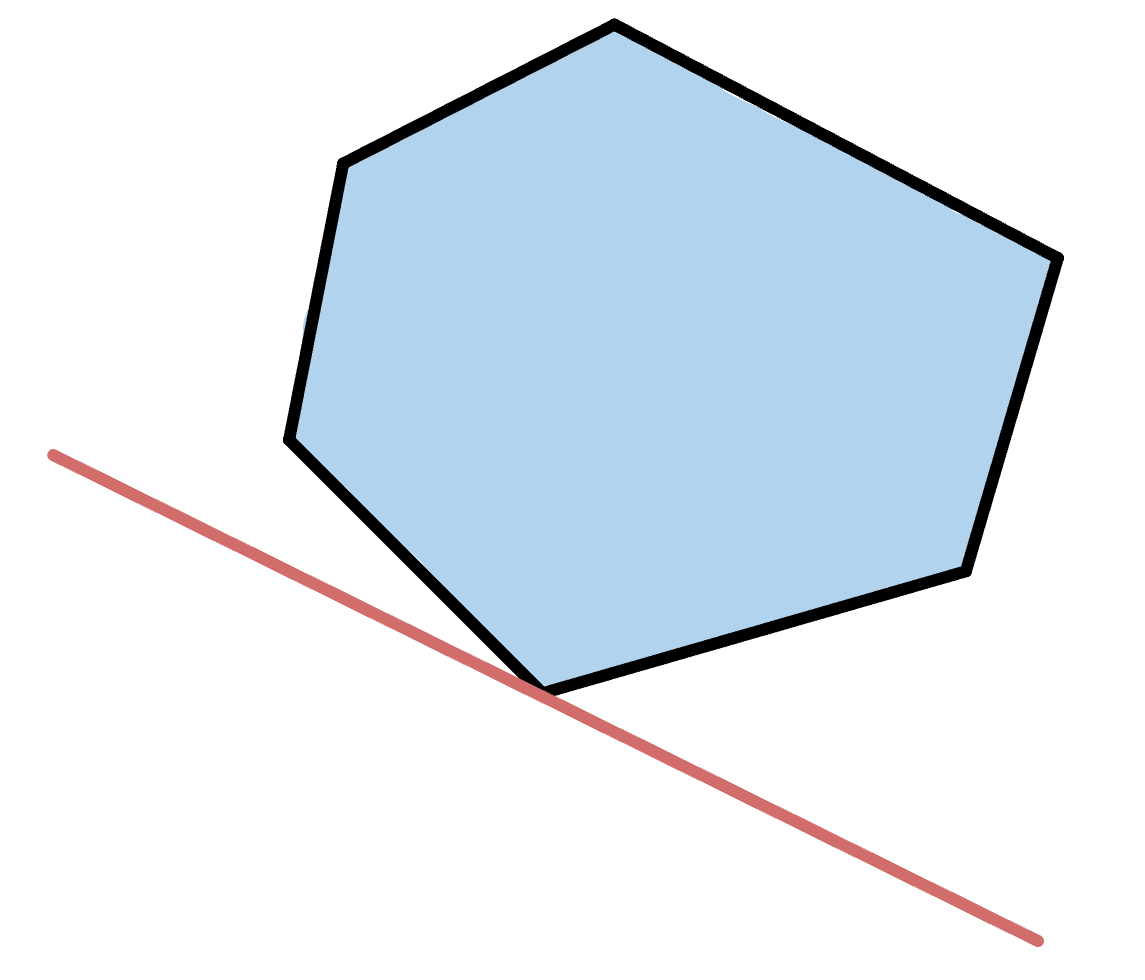
\includegraphics[width=0.375\textwidth]{images/rand_lp.png}
        \end{figure}
        
        \pause
        
        Moreover, if the linear equations have bounded integer coefficients, then evaluation at \textcolor{sigma@alertred}{\textit{small, random}} values has a unique minimum.
    \end{lem}
\end{frame}

\begin{frame}{Isolation Lemma}
    \begin{lem}[{\cite[Lemma 4]{KS01}}]
        Let $\mathcal{L}$ be any collection of distinct linear forms in variables $z_1, \ldots, z_\ell$ with coefficients in the range $\set{0, \ldots, K}$ for some integer $K \in \Z_{\geq 0}$.
        Let $\e > 0$.

        \pause
        \vspace{10pt}
        
        Let $z_1, \ldots, z_\ell$ be independently and uniformly chosen from $\set{0, \ldots, M}$ at random, where $M \geq K \ell / \e$.

        \pause
        \vspace{10pt}

        Then, with probability at least $1 - \e$, there is a unique form in $\mathcal{L}$ of minimum value at $z_1, \ldots, z_\ell$.
    \end{lem}
\end{frame}

\begin{frame}{Isolating Monomials}
    \begin{lem}[{\cite[Corollary 2.27]{DG25}}]
        Consider a polynomial $g(x_1, \ldots, x_\ell)$ such that the individual degree of each $x_i$ in $g$ is at most $K$:
        \[
            g(x_1, \ldots, x_\ell) = \sum_{\overline{e} \in \mathcal{L}} c_{\overline{e}} x_1^{e_1} \cdots x_{\ell}^{e_\ell}.
        \]

        \pause
        
        Randomly choose $z_1, \ldots, z_\ell$ and define a morphism
        \[
            x_i \mapsto w^{z_i} \pause, \qquad g \mapsto \sum_{\overline{e} \in \mathcal{L}} c_{\overline{e}} \cdot w^{\sum_{i = 1}^\ell e_i z_i}.
        \]

        \pause

        The Isolation Lemma shows that the $z_1, \ldots, z_\ell$ can be choose to be small \pause $\implies$ unique lowest $\deg_w$-term \pause and homogenization w.r.t $w$ is small.
    \end{lem}
\end{frame}


\section{Related and Future Work}
\frame{\sectionpage}

\begin{frame}{Pfaffian Analogues}
    \begin{definition}
        If $X$ is a $2n \times 2n$ skew-symmetric matrix,\pause then $\det(X)$ is the perfect square of another polynomial called the \emph{Pfaffian} of $X$.
    \end{definition}

    \pause
    \vspace{20pt}

    \begin{thrm}[{\cite[Theorem 1.6]{DG25}}]
        Let $f \in I^{\pfaff}_{2n, 2r}$ be a nonzero polynomial.
        Then there is a depth-three $f$-oracle circuit of size $\poly(n, \deg(f))$ that \emph{exactly computes} the $t \times t$ pfaffian for some $t = \bigTheta{r^{1 / 3}}$.
    \end{thrm}
    
\end{frame}

\begin{frame}{Symmetric Analogue?}
    The focus on determinantal ideals and pfaffian ideals stem from \emph{invariant theory}.\ \pause
    Are there other natural settings to study from there?

    \pause
    \vspace{20pt}
    
    \begin{question}
        Is there an analogue to our results for the ideal of determinants of a symmetric matrix?
    \end{question}
\end{frame}

\begin{frame}{Roadblocks for the Permanent}
    The other big star in algebraic complexity is the \emph{permanent} of a matrix.
    
    \pause
    \vspace{20pt}
    
    \begin{question}
        Is there an analogue to our results for the ideal of permanents of a matrix?
    \end{question}

    \pause
    \vspace{20pt}

    The main roadblock is that we have no analogue of the following result:
    \[
        (S \mid T)(E_{i, j}(\lambda)X) = \pm \lambda^{h_{i}^{j}(S)} (\Sub_{i \to j}(S) \mid T)(X) + \sum_{h = 0}^{h_{i}^{j}(S) - 1} \lambda^h \sum_{S' \in \mathcal{C}^{h}_{i \to j}(S)} \pm  (S' \mid T)(X).
    \]
\end{frame}

% Quotes are fun, find some to use!
\font\eightss=cmssq8
\font\eightssi=cmssqi8
\newcommand\quoteAuthorDate[2]{\begingroup
  \baselineskip 10pt
  \parfillskip 0pt
  \interlinepenalty 10000 % not needed in example
  \leftskip 0pt plus 40pc minus \parindent
  \let\rm=\eightss
  \let\sl=\eightssi
  \everypar{\sl}#1\par
  \nobreak\smallskip
  \noindent\rm--- #2\unskip\enspace\par
  \endgroup}
% If someone can figure out how to horizontally center this and make the text bigger that'd be cool
\begin{frame}
    \begin{center}
        {\color{sigma@mainblue} \LARGE Thank You!}
    \end{center}
    
    \begin{center}
        \item \quoteAuthorDate{Algebra is generous; she often gives more than is asked of her.}{Jean Le Rond d'Alembert}
    \end{center}

    {\tiny
        Slides can be found on my site \href{https://anakin.phd/}{anakin.phd}
    }
\end{frame}

\begin{frame}[allowframebreaks]{Bibliography}
    \bibliography{refs}
    \bibliographystyle{alpha}
\end{frame}

% Below here is a bunch of template code.

% % Start a section: *sections* (subsections, etc.) are what show up in the TOC.
% \section{Basics}
% % Section pages can be printed thus:
% \frame{\sectionpage}
% 
% \section{Some Template Slides}
% \frame{\sectionpage}
% 
% % Similar for subsections:
% \subsection{A subsection, Wow}
% % And their pages:
% \frame{\subsectionpage}
% 
% \begin{frame}{Image}
%   % This is how you'd include an image, centered.
%   \begin{center}
%     \includegraphics[width=0.25\textwidth]{images/sigma.png}
%   \end{center}
% \end{frame}
% 
% \begin{frame}{Side by Side}
%     \includegraphics[width=0.25\textwidth]{images/sigma.png}\hspace{0.4\textwidth}
%     \includegraphics[width=0.25\textwidth]{images/sigma.png}
% \end{frame}
% 
% \begin{frame}{Demonstration of algo and nalgo env}
%     \begin{algo}
%     \underline{\textsc{GetRandomNumber}():}\+
%     \\      return $4$   \Comment{chosen by fair dice roll.}
%     \\      \hspace{42.75pt}\Comment{guaranteed to be random.}
%     \end{algo}
%     
%     % nalgo has line numbers
%     % only lines with \label{} are numbered
%     \begin{nalgo}[1.3]
%         \underline{\textsc{GetRandomNumber}():}\+
%     \\\label{}  return $4$   \Comment{chosen by fair dice roll.}
%     \\\label{}  \hspace{42.75pt}\Comment{guaranteed to be random.}
%     \end{nalgo}
%     
%     Random number generation from~\cite{site:xkcd}. 
%     \quest{
%     \textbackslash cref for line numbers does not work. 
%     If you want to refer to specific line numbers, do it manually
%     }
%     
% \end{frame}
% 
% \begin{frame}{}
% \begin{minipage}[c]{0.6\textwidth}
% \begin{nalgo}
% \textul{\textbf{\textsc{AlgorithmP}}$(S[a_0, \dots, a_n])$}:
% \\\label{}  $C[1..n] \gets 0, O[1..n] \gets 1$
% \\\label{}  \textbf{while} \textsc{True}:\+
% \\\label{}      \textsc{print}$(S)$
% \\\label{}      {\color{lightgray}$j \gets n, s \gets 0$}
% \\\label{}      {\color{lightgray}\textbf{A:}~~$q \gets C[j] + O[j]$\+}
% \\\label{}          {\color{lightgray}\textbf{if} $q < 0$: goto \textbf{D}}
% \\\label{}          {\color{lightgray}\textbf{if} $q = j$: goto \textbf{B}}
% \\\label{}          {\color{lightgray}\textsc{swap}$(S, j-C[j]+s, j-q+s)$}
% \\\label{}          {\color{lightgray}$C[j] \gets q$} 
% \\\label{}          {\color{lightgray}continue\-}
% \\\label{}      {\color{lightgray}\textbf{B:}~~\textbf{if} $j=1$:\+\+}
% \\\label{}              {\color{lightgray}break\-}
% \\\label{}          {\color{lightgray}$s \gets s+1$\-}
% \\\label{}    {\color{lightgray}\textbf{D:}~~$O[j] \gets -O[j], j \gets j-1$\+}
% \\\label{}      {\color{lightgray}goto \textbf{A}}
% \end{nalgo}
% \end{minipage}
% \begin{minipage}[c]{0.35\textwidth}
% \begin{itemize}
%     \item Here is an example of annotating an algorithms \pause
%     \item We have grayed out text to highlight what we want to discuss 
% \end{itemize}
% \end{minipage}
% \end{frame}
% 
% % Of course, not everything is in pseudocode
% % You MUST have this [containsverbatim] option
% % https://www.overleaf.com/learn/latex/Code_Highlighting_with_minted
% \begin{frame}[containsverbatim]{Source Code}
%     \begin{minted}
%     [
%     framesep=2mm,
%     baselinestretch=1.2,
%     bgcolor=black,
%     fontsize=\footnotesize,
%     ]
%     {python}
%     def algorithm_g(n):
%         a = [0 for _ in range(n + 1)]
%         while True:
%             curr = a[1 : n + 1][::-1]
%             yield "".join([str(i) for i in curr])
%     
%             a[0] = 1 - a[0]
%             j = 1
%             while a[j - 1] != 1:
%                 j += 1
%             if j == n + 1:
%                 return
%             a[j] = 1 - a[j]
%     \end{minted}
% \end{frame}
% 
% 
% \begin{frame}{Theorems and Lemmas}
%     \begin{lem}
%         The map $\C \times \pqty{\C \setminus \set{0}} \to \C$, $(z, w) \mapsto z / w$ is $C^{\infty}$.
%     \end{lem}
%     \begin{pf}
%         To see this, we identify $\C$ with $\R^{2}$ where $a + bi = (a, b)$.
%         Thus our map is now
%         \begin{align*}
%             \pqty{\R^{2}} \times \pqty{\R^{2} \setminus \set{(0, 0)}} &\to \R^{2} \\
%                             ((a, b), (c, d)) &\mapsto \pqty{\frac{ac + bd}{c^{2} + d^{2}}, \frac{bc - ad}{c^{2} + d^{2}}}
%         \end{align*}
%         which is well defined since at least one of $c$ or $d$ is nonzero.
%         It is simple to verify that this map is equivalent to the original one.
%         Since this new map is $C^{\infty}$ in each component, we have that it is $C^{\infty}$ overall.
%     \end{pf}
% \end{frame}
% 
% \section{Conclusion}
% \frame{\sectionpage}
% 
% % Asking questions is fun but we should answer some first
% \begin{frame}{}
%       \begin{center}
%     {\color{sigma@mainblue} \LARGE Questions?}
%   \end{center}
% \end{frame}
% 
% \begin{frame}{Questions!}
%     \begin{itemize}
%         \item How many zeros of $\zeta(s) = \sum\limits_{i = 1}^\infty \frac{1}{n^s} = \prod\limits_{p \text{ prime}} \frac{1}{1 - p^{-s}}$ have real part equal to $\frac{1}{2}$?
%         \item Find a closed form to the following recurrence:
%         $$
%             f(n) = \begin{cases} 
%                 f\pqty{\frac{n}{2}} & n \text{ even} \\
%                 f{3n + 1} & \text{otherwise}                
%             \end{cases}
%         $$
%     \end{itemize}
% \end{frame}
% 

\end{document}
